\documentclass[tikz,border=8pt]{standalone}
\usepackage[T1]{fontenc}\usepackage{lmodern}\usepackage{pgfplots}\pgfplotsset{compat=1.18}
\begin{document}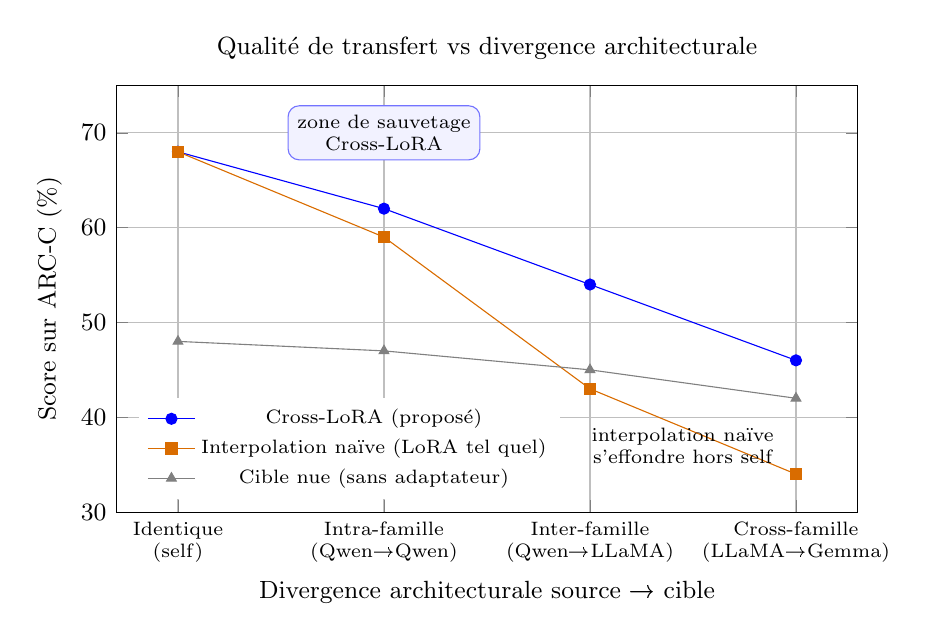
\begin{tikzpicture}
\begin{axis}[width=11cm,height=7cm,font=\small,title={Qualité de transfert vs divergence architecturale},ylabel={Score sur ARC-C (\%)},xlabel={Divergence architecturale source → cible},xmin=.7,xmax=4.3,ymin=30,ymax=75,xtick={1,2,3,4},xticklabels={Identique\\(self),Intra-famille\\(Qwen→Qwen),Inter-famille\\(Qwen→LLaMA),Cross-famille\\(LLaMA→Gemma)},x tick label style={align=center,font=\scriptsize},grid=major,legend pos=south west,legend style={font=\scriptsize,fill=white,draw=none}]
% Conceptual trend redrawn from source; points are schematic, not reported measurements.
\addplot[blue,mark=*] coordinates {(1,68)(2,62)(3,54)(4,46)};\addlegendentry{Cross-LoRA (proposé)}
\addplot[orange!85!black,mark=square*] coordinates {(1,68)(2,59)(3,43)(4,34)};\addlegendentry{Interpolation naïve (LoRA tel quel)}
\addplot[gray,mark=triangle*] coordinates {(1,48)(2,47)(3,45)(4,42)};\addlegendentry{Cible nue (sans adaptateur)}
\node[draw=blue!55,fill=blue!5,rounded corners,font=\scriptsize,align=center] at (axis cs:2.0,70) {zone de sauvetage\\Cross-LoRA};\node[font=\scriptsize,align=center] at (axis cs:3.45,37) {interpolation naïve\\s'effondre hors self};
\end{axis}\end{tikzpicture}\end{document}
